% Beamer slide template prepared by Tom Clark <tom.clark@op.ac.nz>
% Otago Polytechnic
% Dec 2012

\documentclass[10pt]{beamer}
\usetheme{Dunedin}
\usepackage{graphicx}
\usepackage{fancyvrb}

\newcommand\codeHighlight[1]{\textcolor[rgb]{1,0,0}{\textbf{#1}}}

\title{Abstract Data Types}

\author[IN608]{Intermediate Application Development}
\institute[Otago Polytechnic]{
  Otago Polytechnic \\
  Dunedin, New Zealand \\
  Kaiako: Tom Clark
}
\date{}
\begin{document}

%----------- titlepage ----------------------------------------------%
\begin{frame}[plain]
  \titlepage
\end{frame}

%----------- slide --------------------------------------------------%
\begin{frame}
  \frametitle{Abstract Data Types}
   
   An \emph{Abstract Data Type} (ADT) is comprised of two things:
   \begin{itemize}
     \item The set of values which the type can represent;
	 \item The set of operations that can be performed with elements of that type.
   \end{itemize}
   
   It is not concerned with the implementation of the type. Two ADTs that
   represent the same set of the values with the same operations are the same
   ADT.
      
\end{frame}

%----------- slide --------------------------------------------------%
\begin{frame}
  \frametitle{Examples of ADTs}
   
     \begin{itemize}
       \item Stack
	   \item Queue
	   \item Set
	   \item Tree
	   \item Graph
     \end{itemize}
\end{frame}

%----------- slide --------------------------------------------------%
\begin{frame}
  \frametitle{Stack}
  A \emph{stack} is a \textbf{Last in, first out} structure. Think of
  a stack of plates.
  
    \begin{itemize}
       \item Primary operations
          \begin{itemize}
            \item push
            \item pop
          \end{itemize}  
	   \item Additional operations
	      \begin{itemize}
            \item peek
            \item depth (size)
            \item empty
            \item full
          \end{itemize}
     \end{itemize}
\end{frame}

%----------- slide --------------------------------------------------%
\begin{frame}[fragile]
  \frametitle{List as a stack}
   
   \begin{itemize}
       \item List methods
          \begin{itemize}
            \item \texttt{append()} - basically push by another name
            \item \texttt{pop()}
          \end{itemize}  
	   \item See \url{https://docs.python.org/3/tutorial/datastructures.html#using-lists-as-stacks}
	\end{itemize} 
	
	\begin{verbatim}
      stack = []
      print(stack) # []
      stack.append('apple')
      print(stack) # ['apple']
      stack.append('banana')
      print(stack) # ['apple', 'banana']
      stack.append('cherry')
      print(stack) # ['apple', 'banana', 'cherry']
      stack.pop()
      print(stack) # ['apple', 'banana']
    \end{verbatim}  
\end{frame}

%----------- slide --------------------------------------------------%
\begin{frame}[fragile]
  \frametitle{A Stack Class}
   
  	
	\begin{verbatim}
	  class Stack:
          def __init__(self):
              self.stack = []
          def push(self, item):
              pass
          def pop(self):
              pass
          def peek(self):
              pass
          def empty(self):
              pass
              
      stk = Stack()
      stk.push('cat')        
    \end{verbatim}  
\end{frame}

%----------- slide --------------------------------------------------%
\begin{frame}
  \frametitle{Queue}
  A \emph{queue} is a \textbf{First in, first out} structure. Think of
  a queue to check out at a supermarket.
  
    \begin{itemize}
       \item Primary operations
          \begin{itemize}
            \item enqueue
            \item dequeue
          \end{itemize}  
	   \item Additional operations
	      \begin{itemize}
            \item peek
            \item length
            \item empty
            \item full
          \end{itemize}
     \end{itemize}
\end{frame}

%----------- slide --------------------------------------------------%
\begin{frame}[fragile]
  \frametitle{Deque as a queue}
   
   \begin{itemize}
       \item A List is not efficient when used for a queue.
       \item The \texttt{collections} module in the standard library provides a \texttt{Deque}.
       \item Deque methods
          \begin{itemize}
            \item \texttt{append()}
            \item \texttt{popleft()}
          \end{itemize}  
	   \item See \url{https://docs.python.org/3/library/collections.html#collections.deque}
	\end{itemize} 
	
	\begin{verbatim}
      from collections import deque
      queue = deque([])
      print(queue) # deque([])
      queue.append('apple')
      print(queue) # deque(['apple'])
      queue.append('banana')
      print(queue) # deque(['apple', 'banana'])
      queue.append('cherry')
      print(queue) # deque(['apple', 'banana', 'cherry'])
      queue.popleft()
      print(queue) # deque(['banana', 'cherry'])
      
    \end{verbatim}  
\end{frame}

%----------- slide --------------------------------------------------%
\begin{frame}[fragile]
  \frametitle{A Queue Class}
   
  	
	\begin{verbatim}
      from collections import deque
      class Queue:
          def __init__(self):
              self.queue = deque()
          def enqueue(self, item):
              pass
          def dequeue(self):
              pass
          def peek(self):
              pass
          def empty(self):
              pass
              
      q = Queue()
      q.enqueue('cat')        
    \end{verbatim}  
\end{frame}

%----------- slide --------------------------------------------------%
\begin{frame}
  \frametitle{Programming Activity}
  
  \begin{enumerate}
    \item Pull the course materials repo.
    \item Create a new branch, \texttt{03-practical} in your practicals repo.
    \item Add a subdirectory,  \texttt{03-practical} and copy \texttt{03-practical.ipynb} from the class materials into it.
    \item Open a shell, cd to this directory, and run \texttt{jupyter notebook} to open the notebook. Complete the first questions.
    \item We will discuss results in 30ish minutes.
  \end{enumerate}      
\end{frame}

%----------- slide --------------------------------------------------%
\begin{frame}
  \frametitle{Graph}
  A \emph{graph} is made up of a collection of values, called \emph{nodes}, and a
  collection of \emph{edges} that connect two nodes and indicate some sort of relationship between
  the nodes.
  
    
  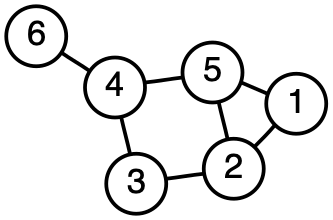
\includegraphics[height=35mm]{6n-graf.png}
  
  
  A special case of a graph is a \emph{tree}.

\end{frame}



\end{document}
